%! Author = zhenxiang
%! Date = 23-3-23

% Preamble
\documentclass[UTF8]{ctexart}

% Packages
\usepackage{amsmath}
% graphicx
\usepackage{graphicx}
% url
\usepackage{hyperref}
\hypersetup{
    colorlinks=true,
    linkcolor=blue,
    filecolor=magenta,      
    urlcolor=cyan,
    pdftitle={标题},
    pdfpagemode=FullScreen,
    }
% 页面设置
\usepackage{geometry}
\geometry{left=2.5cm, right=2.5cm, top=2.5cm, bottom=2.5cm}
% Document
\begin{document}

\section{环境配置}

参考这个网站的
\href{http://doraemonzzz.com/2022/12/25/2022-12-25-ECE408-\%E7\%8E\%AF\%E5\%A2\%83\%E9\%85\%8D\%E7\%BD\%AE\%E4\%BB\%A5\%E5\%8F\%8ALab-0/#Lab-0}{环境配置}\\

实验结果如下
% 图片置于当前位置
\begin{figure}[ht]
    \centering
    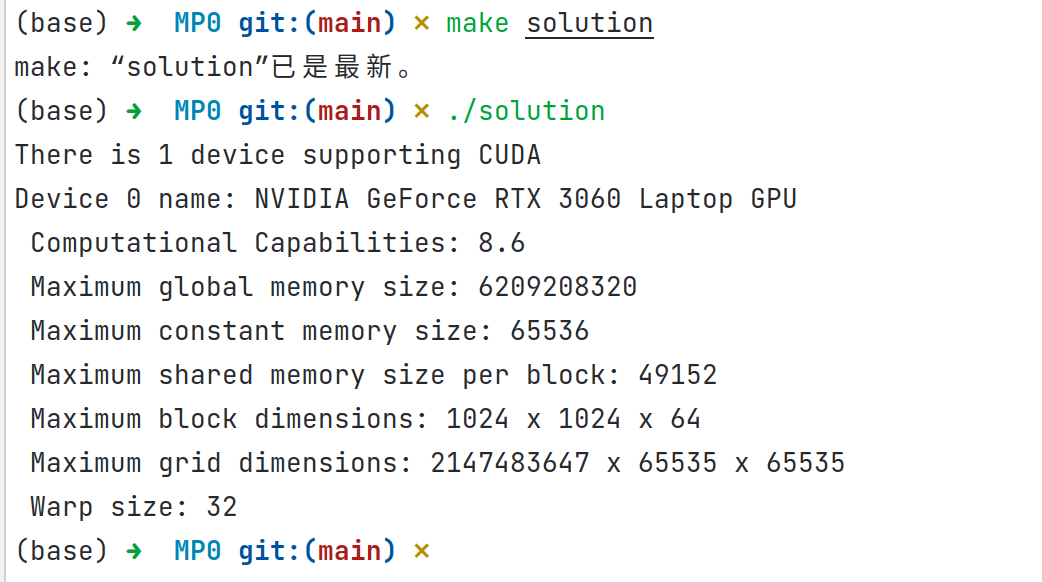
\includegraphics[width=1.0\textwidth]{photos/lab0.png}
    \caption{lab0实验结果}
    \label{fig:1}
\end{figure}



\end{document}